%%%%%%%%%%%%%%%%%%%%%%%%%%%%%%%%%%%%%%%%%
% Lachaise Assignment
% LaTeX Template
% Version 1.1(26/6/2018)
%
% This template originates from:
% http://www.LaTeXTemplates.com
%
% Authors:
% Marion Lachaise & François Févotte
% Vel (vel@LaTeXTemplates.com)
%
% License:
% CC BY-NC-SA 3.0 (http://creativecommons.org/licenses/by-nc-sa/3.0/)
% 
%%%%%%%%%%%%%%%%%%%%%%%%%%%%%%%%%%%%%%%%

%----------------------------------------------------------------------------------------
%	PACKAGES AND OTHER DOCUMENT CONFIGURATIONS
%----------------------------------------------------------------------------------------

\documentclass{article}

%%%%%%%%%%%%%%%%%%%%%%%%%%%%%%%%%%%%%%%%%
% Lachaise Assignment
% Structure Specification File
% Version 1.0 (26/6/2018)
%
% This template originates from:
% http://www.LaTeXTemplates.com
%
% Authors:
% Marion Lachaise & François Févotte
% Vel (vel@LaTeXTemplates.com)
%
% License:
% CC BY-NC-SA 3.0 (http://creativecommons.org/licenses/by-nc-sa/3.0/)
% 
%%%%%%%%%%%%%%%%%%%%%%%%%%%%%%%%%%%%%%%%%

%----------------------------------------------------------------------------------------
%	PACKAGES AND OTHER DOCUMENT CONFIGURATIONS
%----------------------------------------------------------------------------------------

\usepackage{amsmath,amsfonts,stmaryrd,amssymb,bbm,float,graphicx,enumerate,mathtools,listings,xcolor,color,esint,subfig,tikz,pgfplots,adjustbox,setspace,bm,minted,pdfpages,hyperref} % Math packages

\usepackage{enumerate} % Custom item numbers for enumerations

\usepackage[lined,boxed,vlined,ruled]{algorithm2e}
\SetKw{Continue}{continue}
\SetKw{Or}{or}
\SetKw{Until}{until}

\usepackage[framemethod=tikz]{mdframed} % Allows defining custom boxed/framed environments

\usepackage{listings} % File listings, with syntax highlighting
\lstset{
    basicstyle=\ttfamily, % Typeset listings in monospace font
}

\DeclarePairedDelimiter\ceil{\lceil}{\rceil}
\DeclarePairedDelimiter\floor{\lfloor}{\rfloor}

% Allow for the \begin{align} to go over the page
\allowdisplaybreaks

%----------------------------------------------------------------------------------------
%	DOCUMENT MARGINS
%----------------------------------------------------------------------------------------

\usepackage{geometry} % Required for adjusting page dimensions and margins

\geometry{
    paper=a4paper, % Paper size, change to letterpaper for US letter size
    top=2.5cm, % Top margin
    bottom=3cm, % Bottom margin
    left=2.5cm, % Left margin
    right=2.5cm, % Right margin
    headheight=14pt, % Header height
    footskip=1.5cm, % Space from the bottom margin to the baseline of the footer
    headsep=1.2cm, % Space from the top margin to the baseline of the header
    %showframe, % Uncomment to show how the type block is set on the page
}

%----------------------------------------------------------------------------------------
%	FONTS
%----------------------------------------------------------------------------------------

\usepackage[utf8]{inputenc} % Required for inputting international characters
\usepackage[T1]{fontenc} % Output font encoding for international characters

\usepackage{XCharter} % Use the XCharter fonts

%----------------------------------------------------------------------------------------
%	COMMAND LINE ENVIRONMENT
%----------------------------------------------------------------------------------------

% Usage:
% \begin{commandline}
%	\begin{verbatim}
%		$ ls
%		
%		Applications	Desktop	...
%	\end{verbatim}
% \end{commandline}

\mdfdefinestyle{commandline}{
    leftmargin=10pt,
    rightmargin=10pt,
    innerleftmargin=15pt,
    middlelinecolor=black!50!white,
    middlelinewidth=2pt,
    frametitlerule=false,
    backgroundcolor=black!5!white,
    frametitle={Command Line},
    frametitlefont={\normalfont\sffamily\color{white}\hspace{-1em}},
    frametitlebackgroundcolor=black!50!white,
    nobreak,
}

% Define a custom environment for command-line snapshots
\newenvironment{commandline}{
    \medskip
    \begin{mdframed}[style=commandline]
        }{
    \end{mdframed}
    \medskip
}

%----------------------------------------------------------------------------------------
%	FILE CONTENTS ENVIRONMENT
%----------------------------------------------------------------------------------------

% Usage:
% \begin{file}[optional filename, defaults to "File"]
%	File contents, for example, with a listings environment
% \end{file}

\mdfdefinestyle{file}{
    innertopmargin=1.6\baselineskip,
    innerbottommargin=0.8\baselineskip,
    topline=false, bottomline=false,
    leftline=false, rightline=false,
    leftmargin=2cm,
    rightmargin=2cm,
    singleextra={%
            \draw[fill=black!10!white](P)++(0,-1.2em)rectangle(P-|O);
            \node[anchor=north west]
            at(P-|O){\ttfamily\mdfilename};
            %
            \def\l{3em}
            \draw(O-|P)++(-\l,0)--++(\l,\l)--(P)--(P-|O)--(O)--cycle;
            \draw(O-|P)++(-\l,0)--++(0,\l)--++(\l,0);
        },
    nobreak,
}

% Define a custom environment for file contents
\newenvironment{file}[1][File]{ % Set the default filename to "File"
    \medskip
    \newcommand{\mdfilename}{#1}
    \begin{mdframed}[style=file]
        }{
    \end{mdframed}
    \medskip
}

%----------------------------------------------------------------------------------------
%	NUMBERED QUESTIONS ENVIRONMENT
%----------------------------------------------------------------------------------------

% Usage:
% \begin{question}[optional title]
%	Question contents
% \end{question}

\mdfdefinestyle{question}{
    innertopmargin=1.2\baselineskip,
    innerbottommargin=0.8\baselineskip,
    roundcorner=5pt,
    nobreak,
    singleextra={%
            \draw(P-|O)node[xshift=1em,anchor=west,fill=white,draw,rounded corners=5pt]{%
                Question \theQuestion\questionTitle};
        },
}

\newcounter{Question} % Stores the current question number that gets iterated with each new question

% Define a custom environment for numbered questions
\newenvironment{question}[1][\unskip]{
    \bigskip
    \stepcounter{Question}
    \newcommand{\questionTitle}{~#1}
    \begin{mdframed}[style=question]
        }{
    \end{mdframed}
    \medskip
}

%----------------------------------------------------------------------------------------
%	WARNING TEXT ENVIRONMENT
%----------------------------------------------------------------------------------------

% Usage:
% \begin{warn}[optional title, defaults to "Warning:"]
%	Contents
% \end{warn}

\mdfdefinestyle{warning}{
    topline=false, bottomline=false,
    leftline=false, rightline=false,
    nobreak,
    singleextra={%
            \draw(P-|O)++(-0.5em,0)node(tmp1){};
            \draw(P-|O)++(0.5em,0)node(tmp2){};
            \fill[black,rotate around={45:(P-|O)}](tmp1)rectangle(tmp2);
            \node at(P-|O){\color{white}\scriptsize\bf !};
            \draw[very thick](P-|O)++(0,-1em)--(O);%--(O-|P);
        }
}

% Define a custom environment for warning text
\newenvironment{warn}[1][Warning:]{ % Set the default warning to "Warning:"
    \medskip
    \begin{mdframed}[style=warning]
        \noindent{\textbf{#1}}
        }{
    \end{mdframed}
}

%----------------------------------------------------------------------------------------
%	INFORMATION ENVIRONMENT
%----------------------------------------------------------------------------------------

% Usage:
% \begin{info}[optional title, defaults to "Info:"]
% 	contents
% 	\end{info}

\mdfdefinestyle{info}{%
topline=false, bottomline=false,
leftline=false, rightline=false,
nobreak,
singleextra={%
\fill[black](P-|O)circle[radius=0.4em];
\node at(P-|O){\color{white}\scriptsize\bf i};
\draw[very thick](P-|O)++(0,-0.8em)--(O);%--(O-|P);
}
}

% Define a custom environment for information
\newenvironment{info}[1][Info:]{ % Set the default title to "Info:"
    \medskip
    \begin{mdframed}[style=info]
        \noindent{\textbf{#1}}
        }{
    \end{mdframed}
}

\pgfplotsset{compat=1.12}
\usepgfplotslibrary{fillbetween}
\DeclareMathOperator{\sech}{sech}
\DeclareMathOperator{\arcsech}{arcsech}
\DeclareMathOperator{\arcoth}{arcoth}
\DeclareMathOperator{\arctanh}{tanh^{-1}}
\renewcommand{\baselinestretch}{1.25}
\newcommand{\bin}{{\sf Bin}}
\newcommand{\G}{{\sf G}}
\newcommand{\Hyp}{{\sf Hyp}}
\newcommand{\Ber}{{\sf Ber}}
\newcommand{\Po}{{\sf Po}}
\newcommand{\Poi}{{\sf Poi}}
\newcommand{\ex}{{\sf Exp}}
\newcommand{\Nor}{{\sf N}}
\newcommand{\gam}{{\sf Gam}}
\newcommand{\Em}{\mathbb E}
\newcommand{\Pm}{\mathbb P}
\newcommand{\R}{\mathbb R}
\newcommand{\Cm}{\mathbb C}
\newcommand{\B}{\cal B}
\newcommand{\F}{\mathbb F}
\newcommand{\N}{\mathbb N}
\newcommand{\Z}{\mathbb Z}
\newcommand{\Q}{\mathbb Q}
\newcommand{\Comp}{\mathbb C}
\newcommand{\e}{\mbox{e}}
\newcommand{\Var}{\mbox{Var}}
\newcommand{\cov}{\mbox{Cov}}
\newcommand{\ds}{\displaystyle}
\newcommand{\subvect}[1]{\mbox{\small \boldmath #1}}
%\newcommand{\vect}[1]{\mbox{\boldmath $#1$}}
\newcommand{\vect}[1]{\boldsymbol #1}
\newcommand{\norm}[1]{\left\lVert#1\right\rVert}
\newcommand*\VF[1]{\mathbf{#1}}
\newcommand*\dif{\mathop{}\!\mathrm{d}}
\setlength{\jot}{7pt}
\definecolor{lbcolor}{rgb}{0.95,0.95,0.95}

\title{COMP4702: 2021 Final Exam} % Title of the assignment

\author{Michael Ciccotosto-Camp\\ \texttt{s4430291}} % Author name and email address

\date{University of Queensland --- \today}
\begin{document}

\maketitle % Print the title

% \section*{Data Edits Visualizations}

% \begin{itemize}
%     \item What changes where made to the dataset. Were rows/columns removed or edited? Why?
%     \item What any standardization/normalization performed?
%     \item Does the data look easy to separate when projected onto a lower dimension using PCA,TSNE, etc? How might this influence which model we use?
%     \item Graph the covariances between the data.
% \end{itemize}

To start rows that contained Nan values where removed from the data set so that all the features could be utilized for prediction. Columns with non-numerical (i.e species, island and sex) where numerical encoded using sklearns label encoder. Next the "island" column was drop as this. To justify this notice the spree graph before and after the "island" column is dropped.

\begin{figure}[H]
    \centering
    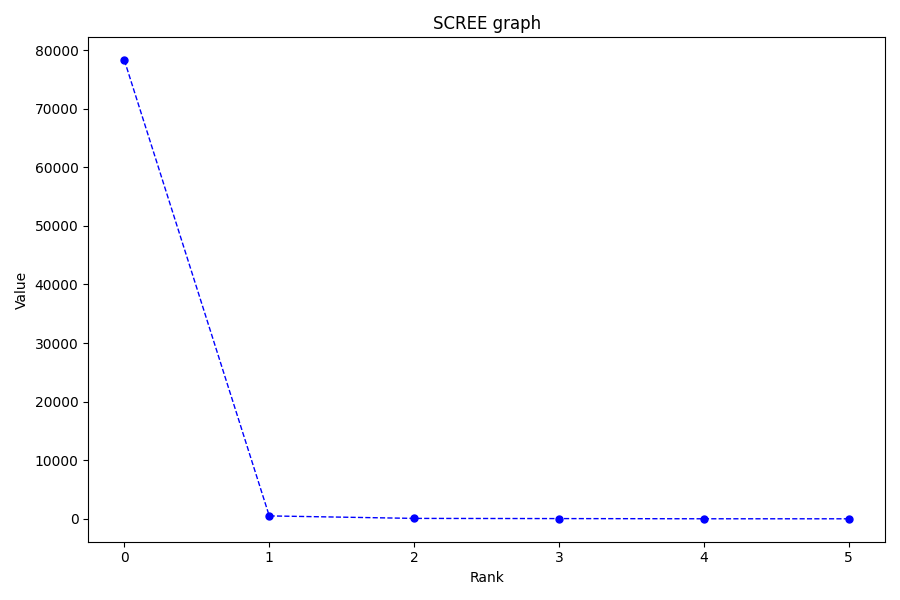
\includegraphics[scale=0.5]{scree_island.png}
    \caption{SPREE graph with island retained}
\end{figure}

\begin{figure}[H]
    \centering
    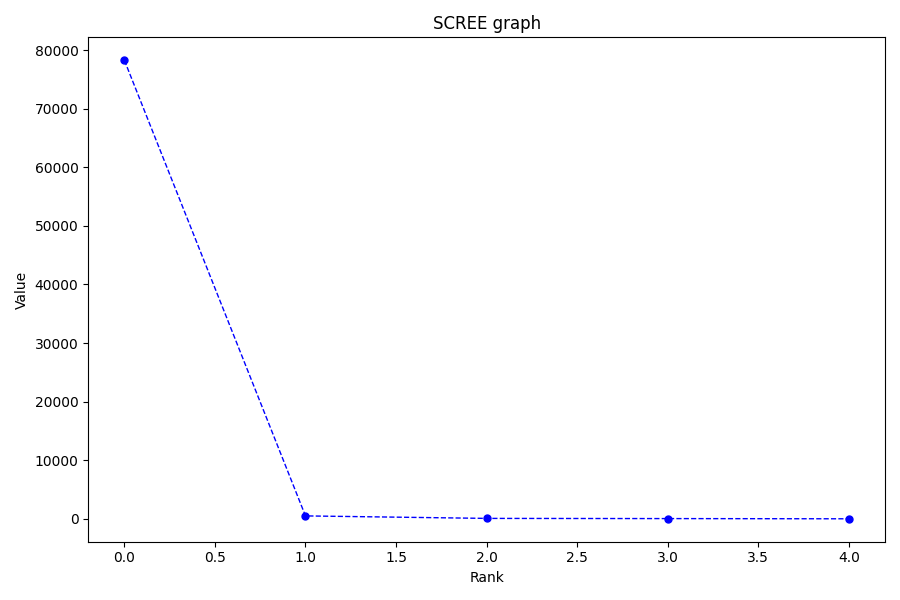
\includegraphics[scale=0.5]{scree_no_island.png}
    \caption{SPREE graph with island removed}
\end{figure}

The fact that the importance weighting of principal components remains relatively unaffected indicates the island feature contributed very little information. Another thing to notice is that the vast majority of importance weighting in the spree graph resides in the first principal component. This suggests that the data undergo further dimensionality reduction without too much feature information loss. This is supported by the fact that there are a number of correlations depicted in the boxplots and covariance matrix.

\begin{figure}[H]
    \centering
    
\includegraphics[scale=0.6]{bp_1.png}
\end{figure}

\begin{figure}[H]
    \centering
    
\includegraphics[scale=0.6]{bp_2.png}
\end{figure}

\begin{figure}[H]
    \centering
    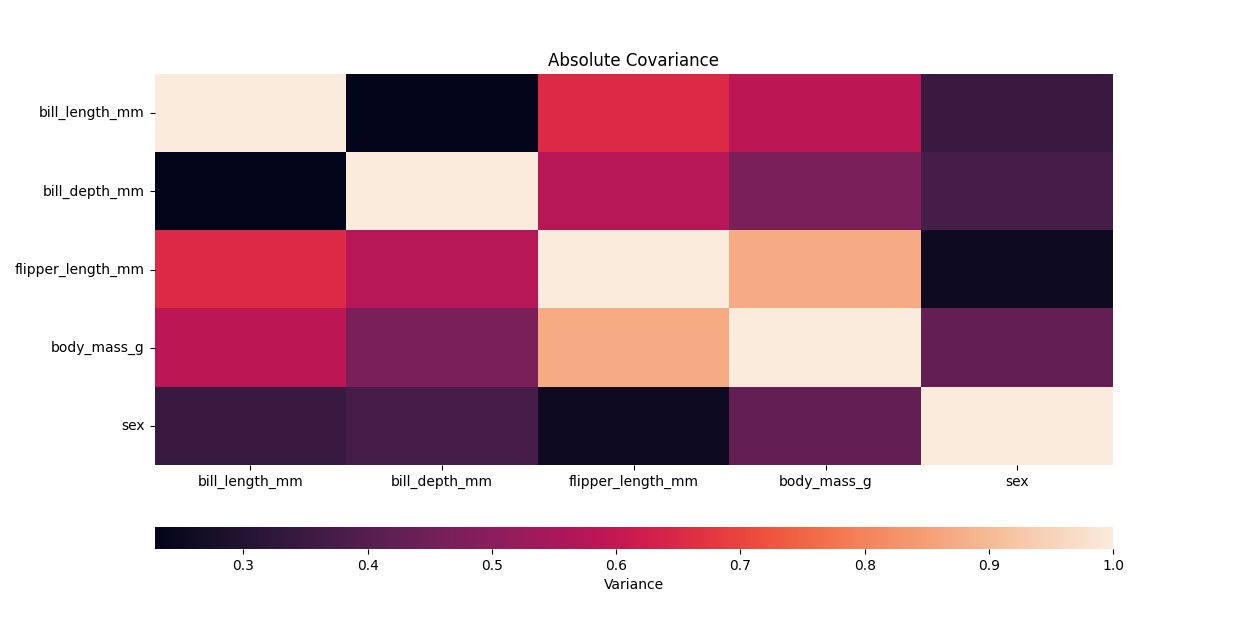
\includegraphics[scale=0.4]{cov_feat_mat.png}
    \caption{Covariance matrix between continuous features}
\end{figure}

A number of dimensionality reduction techniques were used project the data onto a 2-dimensional to see how well they separate out the data. Each feature was standardized before hand so that the dimensionality reduction techniques so that no feature had a information retention weighting. The techniques used were PCA, TSNE and LDA. The results are presented below.

\begin{figure}[H]
    \centering
    
\includegraphics[scale=0.7]{projection_PCA.png}
\end{figure}

\begin{figure}[H]
    \centering
    
\includegraphics[scale=0.7]{projection_TSNE.png}
\end{figure}

\begin{figure}[H]
    \centering
    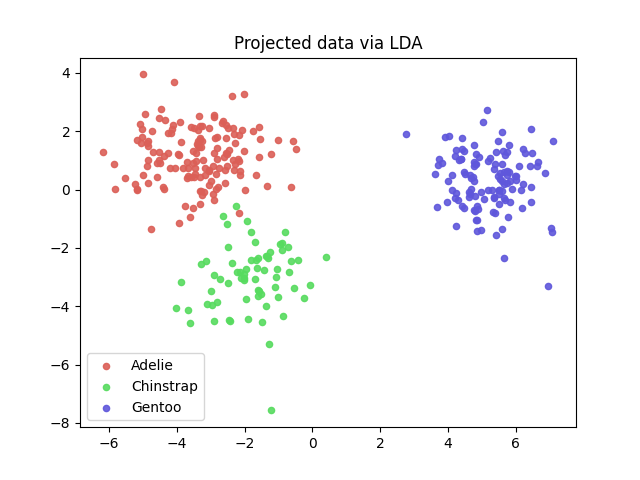
\includegraphics[scale=0.7]{projection_LDA.png}
\end{figure}

TSNE was chosen to be the preferred method for dimensionality reduction since it seemed to provide the best separation between classes and seems to also provide separation between genders (which was not really being tested here, but was still interesting).

% \section*{Model Selection}

% \begin{itemize}
%     \item What model was chosen? Explain why the selected model is suitable for the task at hand (eg its a good idea use SVC if a classification problem is given to us and all the inputs are continuous).
%     \item What parameters were selected? Were they adjusted/how?
% \end{itemize}

An SVM model was chosen since SVMs are designed to perform classification tasks on continuous inputs. The RBF kernel was used as the kernel parameter since, when looking at the TSNE projection, each cluster vaguely resembles a circle where it becomes more and more unlikely to find samples belong to that cluster the further you are from the clusters centre. The default length parameter of the kernel was used. The result for the SVM model comparing true labels and predicted labels and the confusion matrix are presented below.

\begin{figure}[H]
    \centering
    
\includegraphics[scale=0.7]{true_vs_pred.png}
\end{figure}

\begin{figure}[H]
    \centering
    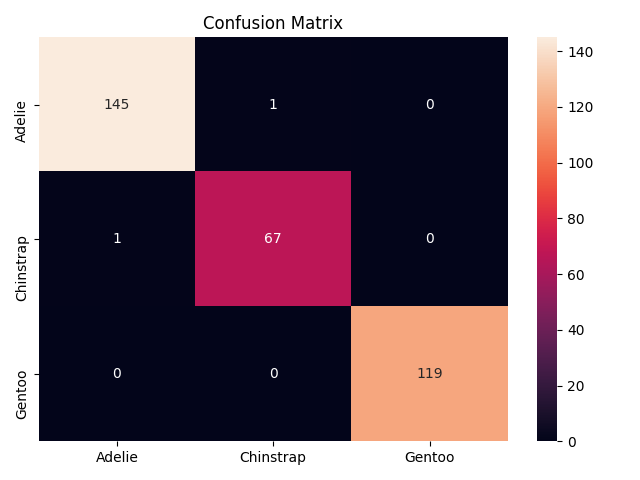
\includegraphics[scale=0.7]{confusion_mat.png}
\end{figure}

As we can see the model was mostly very successfully although, from the confusion matrix, we can see that one misclassification was made between the Chinstrap and Adelie species. This is sort of expected since, in the TSNE graph we see that one Chinstrap is very close to a Adelie cluster centre.

% \section*{Results}

% \begin{itemize}
%     \item For a classification problem, graph out a confusion matrix. How might the data projects onto lower dimensions explain confusion between certain classes. If two classes to closer together when projected onto a lower dimension, then there is a good chance that the model may mistake them.
%     \item Graph how the true outputs compare to the predicted outputs.
%     \item What other improvements to the model could be made if more time was allowed?
% \end{itemize}

\end{document}